\section{KG Selection Framework}
\label{app:kg_selection_framework}
\begingroup
\setlength\tabcolsep{0pt}
\titleformat{\subsubsection}[block]{\large\bfseries}{\thesubsubsection}{3mm}{}

This section contains a detailed description of use of the \gls{kg} selection framework introduced in \cite{farber2017dataquality}.
The analyzed \glspl{kg} are DBPEDIA, FreeBase, OpenCyc, WikiData \cite{vrandecic2014wikidata}, and YAGO \cite{mahdisoltani2015YAGO3} which were included in the original framework.
%The \glspl{kg} WordNet, ICEWS, and GDELT have been added as they are prevalent in the related work.
The result of the analysis is available in \autoref{tab:selection_framework}.

\begin{table*}[ht]
\centering
\begin{minipage}{0.95\textwidth}
\centering
\small
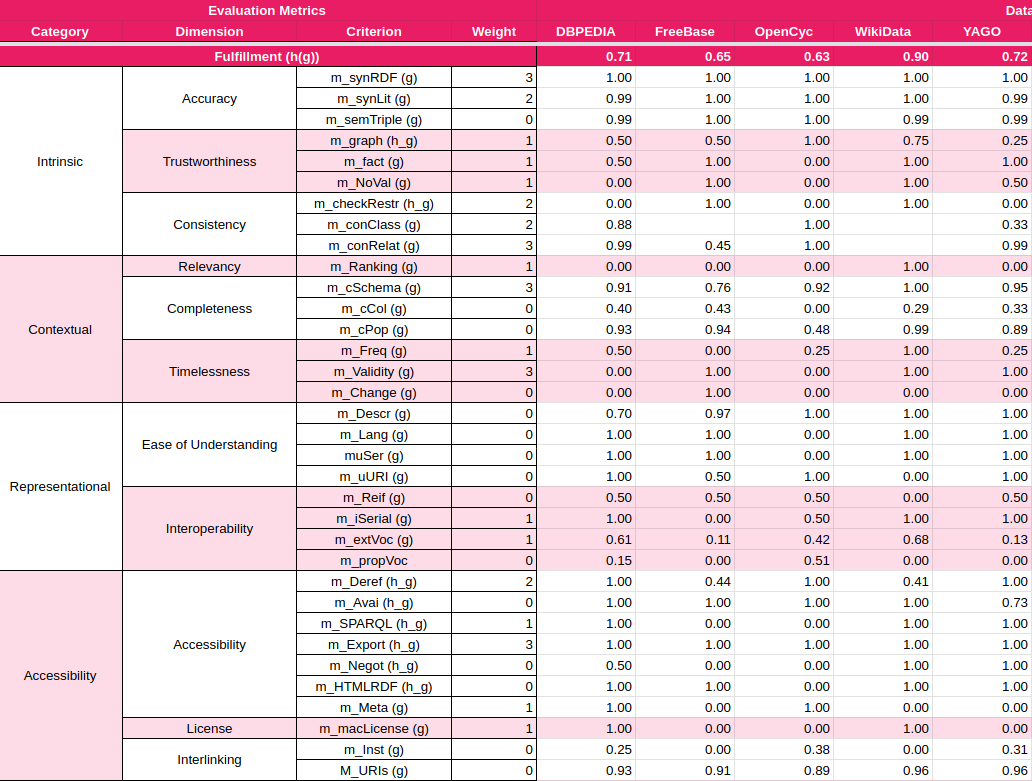
\includegraphics[scale=0.5]{content/appendix/figures/image.png}
\caption{Values for DBPEDIA, FreeBase, OpenCyc, WikiData and YAGO are taken from \cite{farber2017dataquality} as a rule. Exceptions are marked with '*' and explained in \autoref{app:kg_selection_framework}.
%Values for WordNet, ICEWS and GDELT are added \missing
}
\renewcommand{\arraystretch}{1.2}

\begin{comment}
\begin{tabular}{|m{2.5cm}|M|c|c|c|c|M|c|}
\hline
\thead{Method} & %method
\thead{Category} & %category
\thead{Temporal\\Information} & %temporal
\thead{Symmetric\\Relations} & %symmetry
\thead{Anti-\\Symmetric\\Relations} & %anti-symmetry
\thead{Entity\\Embedding} & %entity embedding
%\thead{Relation Embedding} & %relation embedding
\thead{Time\\Dimension} & %time dimension
\thead{Space} %space
\\
\hline
%\rowcolor{blue!10}
TransE \newline\cite{transe} & %method
Transformation \newline (translation) & %category
 & %temporal
 & %symmetry
\checkmark & %anti-symmetry
Separate & %entity embedding
%Single Vector & %relation embedding
\hrulefill & %time dimension
$\R$%space
\\
\hline
\end{tabular}
\end{comment}

\label{tab:selection_framework}
\end{minipage}
\end{table*}

Weights are assigned based on the perceived importance of a criterion relative to the project. They are determined as follows:
\begin{enumerate}
    \setcounter{enumi}{-1}
    \item Irrelevant
    \item Interesting, but most likely irrelevant
    \item Important
    \item Central
\end{enumerate}

In the following is given: a short description of each criterion; the assigned weight; reasoning behind the weight; notes where values have been changed from the original framework.

\subsection{Intrinsic Category}
The intrinsic category describes the data quality independent of the context.

\subsubsection{Accuracy}
The accuracy dimension describes whether the data is without errors.


\weighttable
{m_{synRDF(g)}}
{The syntactic validity of RDF documents.}
{3}
{Syntactic validity is necessary for machine interpretation and machine interpretation is necessary to train a model. As it is unrealistic to fix errors manually it is central that the documents are syntactically valid.}
{}

\weighttable
{m_{synLit}(g)}
{The syntactic validity of literals dependent on data types or pre-defined regular expressions.}
{2}
{The syntactic validity of literals is important as inconsistencies presumably affects the models negatively and we aim to analyze the models at their optimal performance. However it is possible to train the models and obtain a result even with syntactic invalidity in literals and as such it is not as important as $m_synRDF(g)$, the syntactic validity of documents.}
{The value for $m_{synLit}(YAGO)$ was changed from 0.62 to 0.99. The low value was due to YAGO allowing wildcards in the date datatype. As this is a feature in our context, the value was dismissed and an estimate was made based on the remaining factors.}

\weighttable
{m_{semTriple}(g)}
{The degree to which facts hold true.}
{0}
{The purpose of an embedding model is to represent available data and the performance of the model is evaluated against that same data. As such it is irrelevant whether the data holds true or not outside of the \gls{kg}.}
{}

\subsubsection{Trustworthiness}
The Trustworthiness dimension describes whether the data is credible.

\weighttable
{m_{graph}(h_g)}
{Trustworthiness on \gls{kg} level measured by manner of insertion and curation.}
{1}
{This criterion prioritizes manual over automatic work and experts over community. 
While we believe that this approach values the more reliable data higher and we acknowledge that the quality of training data highly impacts the quality of the resulting models, it is also noted that automatic means tend to yield bigger datasets, which also highly impacts the quality of the resulting models. Based on the assumption that significant problems will be revealed through other criteria we consider this criterion interesting, but likely irrelevant.}
{}

\weighttable
{m_{fact}(g)}
{Triples or documents are connected to sources}
{1}
{It lends credibility to the graph and is likely useful in a production setting, but while it is interesting, it is probably irrelevant as it is not the focus of the project and thus likely won't be of use.}
{}

\weighttable
{m_{NoVal}(g)}
{Indication of unknown and empty values}
{1}
{Could be used for negative sampling, as samples that are close to the truth are more valuable than those that are not \cite{yang2020negative-sampling, hyunh2019fact-checking-benchmark}. While this could help identification of those samples and negative sampling could improve model performance, it is not the focus of the project, probably won't be used and is thus interesting, but likely irrelevant.}
{The value for $m_{NoVal}(YAGO)$ was changed from 0 to 0.5 as YAGO does have some capacity for storing this information, through relations and use of wildcards to represent uncertainty.}

\subsubsection{Consistency}
The consistency dimension describes whether the data conflicts with itself.

\weighttable
{m_{checkRestr}(h_g)}
{Whether schema restrictions are checked at insertion time.}
{2}
{In general it is important that the data is consistent in order to enable models to properly represent the information.}
{}

\weighttable
{m_{conClass}(g)}
{Whether class restrictions are upheld.}
{2}
{It is important that class restrictions are upheld in order to eliminate possible sources of error, but as no hypothesis directly concerns class restrictions it is not central.}
{The values for $m_{conClass}(FreeBase)$ and $m_{conClass}(WikiData)$ are dismissed as the inspected constraints are not available in those graphs.}

\weighttable
{m_{conRelat}(g)}
{Whether relation restrictions are upheld.}
{3}
{As hypothesis \missing concerns model ability to represent various relations it is central that the relation constraints are upheld in the data.}
{The value for $m_{conClass}(WikiData)$ is dismissed as the inspected constraint is not available in that graph.}

\subsection{Contextual}
The contextual category describes the data quality in relation to the context.

\subsubsection{Relevancy}
The relevancy dimension describes whether the data is relevant to the purpose.

\weighttable
{m_{Ranking}(g)}
{Ranking of fact importance relative to one another}
{1}
{Could be used to extract more meaningful positive samples or when training models with an attention mechanism. However neither of those are the focus of this project and the information is thus interesting, but likely irrelevant.}
{The source is inconsistent in reports of $m_{Ranking}(FreeBase)$ and reports both 0 and 1. The 0 value is selected as it is consistent with the textual analysis and the values reported for remaining \glspl{kg}.}

\subsubsection{Completeness}
The completeness dimension describes whether the data is missing information relevant to the purpose.

\weighttable
{m_{cSchema}(g)}
{Quantifies missing classes and relations}
{3}
{As certain classes and relation are the subject of several analyses it is central that those classes and relations are present in the data. This is elaborated in \missing.}
{}

\weighttable
{m_{cCol}(g)}
{Quantifies missing relations on instances of classes}
{0}
{It is both an accepted reality and the point of the link prediction task that some information will be missing. While the total number of instances per relation is important, the degree to which entities are annotated with all entities is irrelevant.}
{}

\weighttable
{m_{cPop}(g)}
{Quantifies missing instances}
{0}
{This is irrelevant as the analysis concerns models' ability to embed data with certain characteristics rather than exact data.}
{}

\subsubsection{Timelessness}
The timelessness dimension describes whether the age af data is suitable for the purpose.

\weighttable
{m_{Freq}(g)}
{Frequency of updates}
{1}
{Data should be current to the extent that it is represented in current research to enable comparison of results and ease implementation efforts.}
{}

\weighttable
{m_{Validity}(g)}
{Specification of temporal validity}
{3}
{The project is focused on temporal embedding methods and as such the availability of temporal information is central to the analysis.}
{}

\weighttable
{m_{Change}(g)}
{Specification of last modification}
{0}
{In order to eliminate possible sources of error models are trained on static datasets and as such the modification date is irrelevant.}
{}

\subsection{Representational}
The representational category describes the format of data.

\subsubsection{Ease of Understanding}
The ease of understanding dimension describes whether the data is without ambiguity for a human.

\weighttable
{m_{Descr}(g)}
{Entities are labelled with descriptions.}
{0}
{The models do not need this information to train and the information is not valuable in the context of any hypotheses. As such it is irrelevant.}
{}

\weighttable
{m_{Lang}(g)}
{Contains labels in multiple languages}
{0}
{The models do not need this information to train and the information is not valuable in the context of any hypotheses. As such it is irrelevant.}
{}

\weighttable
{m_{uSer}(h_g)}
{More human-readable serialization formats are available.}
{0}
{The \gls{kg} used as input is not examined beyond its fulfillment of data quality requirements which are analyzed here. As such it is irrelevant whether it is human-readable or not.}
{}

\weighttable
{m_{uURI}(g)}
{Short, self-describing, non-generic URIs.}
{0}
{Though the value of immediately interpretable URIs to the human reader is obvious the value of clearly distinguishable URIs should not be dismissed and as the interpretation is available through labels the short URIs are irrelevant.}
{}

\subsubsection{Interoperability}
The interoperability dimension describes whether the data is without ambiguity for a computer.

\weighttable
{m_{Reif}(g)}
{Avoidance of blank nodes and reification statements.}
{0}
{The usage of blank nodes and reification statements could both improve and impair model performance. As it is not immediately obvious what impact their use has on model performance it is not possible to select the option allowing better model performance and as no hypothesis concerns this aspect whether they are used or not is irrelevant.}
{The source is inconsistent in its reports of $m_{Reif}(DBPEDIA)$ and reports both values of 0.5 and 1. The 0.5 value is selected as it is consistent with the textual analysis and the values reported for remaining \glspl{kg}.}

\weighttable
{m_{iSerial}(g)}
{The availability of other serialization formats.}
{1}
{Embedding methods typically require the input data in the format of tuples. While it is convenient to have the data supplied in the right format converting it is simple as long as it is syntactically valid and as such the availability of other formats is interesting, but likely irrelevant.}
{}

\weighttable
{m_{extVoc}(g)}
{Usage of external vocabulary for relations.}
{1}
{Multiple \glspl{kg} are analyzed in order to generalize observations. If all sources used the same vocabulary it would allow more fine-grained analysis and might simplify parts of the analysis, but the focus of our analysis is generally of a higher abstraction level and thus external vocabulary is interesting, but likely irrelevant.}
{The source is inconsistent in its reports of $m_{extVoc}(OpenCyc)$ and reports both values of 0.415 and 0.41. As this appears to be a rounding error the value 0.415 is used.}

\weighttable
{m_{propVoc}(g)}
{Linking the vocabulary to that of external sources.}
{0}
{In principle the reasoning is very similar to that of $m_{extVoc}(g)$. However this adds an additional layer of complexity to an already unlikely task, making the information irrelevant.}
{}

\subsection{Accessibility}
The accessibility category describes the accessibility of the data.

\subsubsection{Accessibility}
The accessibility dimension describes whether the data is available as well as the ease and speed of retrieval.

\weighttable
{m_{Deref}(h_g)}
{URIs are resolvable via HTTP requests.}
{2}
{It is important to have access to additional information about the resources in order to discover patterns.}
{The source has switched the values of $m_{Deref}(h_{FreeBase})$ and $m_{Deref}(h_{OpenCyc})$ in at least one instance. $m_{Deref}(h_{FreeBase})$ is set to 0.437 and $m_{Deref}(h_{OpenCyc})$ is set to 1 as those are the most commonly reported numbers and consistent with the textual analysis.}

\weighttable
{m_{Avai}(h_g)}
{Uptime of the \gls{kg}.}
{0}
{As only static data is queried it is irrelevant.}
{The source has switched the values of $m_{Avai}(h_{FreeBase})$ and $m_{Avai}(h_{YAGO})$ in at least one instance. $m_{Avai}(h_{FreeBase})$ is set to 0.9998 and $m_{Avai}(h_{YAGO})$ is set to 0.7306 as those are the most commonly reported numbers and consistent with the textual analysis.}

\weighttable
{m_{SPARQL}(h_g)}
{The availability of a SPARQL endpoint.}
{1}
{In a production setting this would likely be necessary, but as that is outside the scope of this project it is interesting, but likely irrelevant.}
{The source has switched the values of $m_{SPARQL}(h_{FreeBase})$ and $m_{SPARQL}(h_{YAGO})$ in at least one instance. $m_{SPARQL}(h_{FreeBase})$ is set to 0 and $m_{SPAQRL}(h_{YAGO})$ is set to 1 as those are the most commonly reported numbers and consistent with the textual analysis.}

\weighttable
{m_{Export}(h_g)}
{The ability to export the data in RDF format.}
{3}
{In order to eliminate possible sources of error models are trained on static datasets which are exported from the \gls{kg} and the ability to so is therefore central.}
{}

\weighttable
{m_{Negot}(h_g)}
{Support of content negotiation that is dereferencing sources in client's preferred serialization format.}
{0}
{As long as content is returned in a valid serialization format the exact format is largely irrelevant.}
{The source has switched the values of $m_{Negot}(h_{FreeBase})$ and $m_{Negot}(h_{YAGO})$ in at least one instance. $m_{Negot}(h_{FreeBase})$ is set to 0 and $m_{Negot}(h_{YAGO})$ is set to 1 as those are the most commonly reported numbers and consistent with the textual analysis.}

\weighttable
{m_{HTMLRDF}(h_g)}
{Linking HTML descriptions and RDF serializations to facilitate automatic link discovery.}
{0}
{While possibly useful to improve the performance of embedding models, we are unaware of any embedding methods utilizing it and it is therefore irrelevant.}
{The source has switched the values of $m_{HTMLRDF}(h_{OpenCyc})$ and $m_{HTMLRDF}(h_{YAGO})$ in at least one instance. $m_{HTMLRDF}(h_{OpenCyc})$ is set to 0 and $m_{HTMLRDF}(h_{YAGO})$ is set to 1 as those are the most commonly reported numbers and consistent with the textual analysis.}

\weighttable
{m_{Meta}(g)}
{Machine-readable metadata via sitemaps and VoID.}
{1}
{Some embedding methods make use of metadata to improve the performance of the model. As this aspect is not covered in any hypothesis, the information is interesting, but likely irrelevant.}
{The source has switched the values of $m_{Meta}(OpenCyc)$ and $m_{Meta}(YAGO)$ in at least one instance. $m_{Meta}(OpenCyc)$ is set to 1 and $m_{Meta}(YAGO)$ is set to 0 as those are the most commonly reported numbers and consistent with the textual analysis.}

\subsubsection{License}
The license dimension describes the license the data is subject to.

\weighttable
{m_{macLicense}(g)}
{Availability of machine-readable license.}
{1}
{It is important that there is a license permitting our use of the data but as a human-readable version is sufficient it is interesting, but likely irrelevant whether a machine-readable one exists.}
{}

\subsubsection{Interlinking}
The interlinking dimension describes whether data representing the same entities is linked.

\weighttable
{m_{Inst}(g)}
{Equivalence links to external sources.}
{0}
{This would only be relevant if models were trained on combined graphs. As that is not the case it is irrelevant.}
{The source is inconsistent in its reports of $m_{Inst}(DBPEDIA)$ and $m_{Inst}(OpenCyc)$. $m_{Inst}(DBPEDIA)$ is reported as 0.592 and 0.251 and $m_{Inst}(OpenCyc)$ is reported as 0.443 and 0.382.
$m_{Inst}(DBPEDIA)$ is set to 0.251 and $m_{Inst}(OpenCyc)$ is set to 0.382 as those are the most commonly reported numbers and consistent with the textual analysis.}

\weighttable
{m_{URI}(g)}
{Validity of of external URIs.}
{0}
{This is irrelevant as the external URIs are not used.}
{The source is inconsistent in its reports of $m_{URI}(DBPEDIA)$ and $m_{URI}(FreeBase)$ and the textual analysis does not resolve these inconsistencies. $m_{URI}(DBPEDIA)$ is set to 0.929 and $m_{URI}(FreeBase)$ is set to 0.908 as those are the most common values. It is also noted that greatest value difference is 0.06.}
\endgroup